\chapter{Transformata Fourier pentru găsirea regiunilor cu anomalii}

\section{Scopul metodei}

Putem folosi această metodă pentru a găsi regiuni cu puncte anormale dintr-o serie de timp, anume regiuni în care punctele 
au caracteristici similare doar că foarte diferite faţă de vecinii lor din afara regiunii \cite{10.5555/1789574.1789615}.


Vom utiliza această idee doar pentru găsirea anomaliilor în date înregistrate în trecut, fapt ce ne-ar ajuta să analizăm 
impactul pe care anumite evenimente l-au avut asupra bursei de valori, precum o criză economică, şi astfel am putea prezice 
mai bine în viitor ce efect ar avea un eveniment similar. Metoda nu are ca scop prezicerea unor noi valori 
de pe bursă.

\section{Ideea din spatele metodei}

Transformata Fourier presupune că semnalul pe care îl analizează este \textbf{periodic} sau măcar foarte apropiat 
de unul periodic. Astfel, ar fi posibil să modelăm acest semnal folosind o sumă de sinusoide de frecvenţe diferite 
pentru seriile de timp complexe sau chiar cu o singură sinusoidă în cazul banal.

Aplicăm transformata Fourier pe seria de timp dată, iar apoi inversăm operaţia doar că vom păstra doar un număr $p$
de parametri, practic presupunâd ca \textbf{magnitudinea frecvenţelor} corespunzătoare este 0. Alegem să păstrăm doar primii 
$p$ parametri cu magnitudinile cele mai mari.

Apoi, folosind acest semnal, calculăm diferenţele între valorile eşantioanelor de pe aceeaşi poziţie(înregistrate la aceeaşi dată)
a ambelor semnale. Punctele care au o diferenţă absolută mai mare decât media diferenţelor absolute pentru toate punctele vor fi considerate
\textbf{potenţiale} anomalii. Pentru aceste potenţiale anomalii vom păstra într-un set $S$ diferenţa dintre valoarea seriei în punctul respectiv 
şi media a $c$ vecini ai săi de pe ambele părţi. Aplicăm \textbf{z-score} pentru fiecare punct din setul $S$, iar punctele a căror valoare 
depăşeşte un prag predefinit $t$ sunt considerate anomalii. Pentru găsirea regiunilor anormale, găsim 2 puncte consecutive cu z-score 
de \textbf{semn opus} care vor marca începutul regiunii, iar pentru a marca finalul, găsim 2 puncte consecutive cu z-score de semn opus, doar 
că în ordine inversă faţă de semnele care marchează începutul.

Punctele cu z-score pozitiv sunt asociate cu \textbf{vârfuri}, în timp ce cele cu semn negativ sunt asociate \textbf{văilor}. Din acest motiv,
acest algoritm funcţionează cel mai bine atunci când datele suferă schimbări \textbf{bruşte în frecvenţă}. Dacă schimbările se întâmplă gradual,
este posibil să nu mai găsim aceste diferenţe majore pentru z-score care să ne indice regiunile cu anomalii. Cu toate acestea, complexitatea 
de timp scăzută a algoritmului, anume $O(n \log n)$ datorită transformării Fourier rapide, face această metodă atractivă atunci când 
eficienţa este un criteriu important.

\section{Reprezentarea matematică}

\[ X[k] = \sum_{n=0}^{N-1} x[n] \cdot e^{-j\frac{2\pi}{N}kn} \]

\[ y[n] = \frac{1}{N} \sum_{k=0}^{N-1} X[k] \cdot e^{j\frac{2\pi}{N}kn} \] cu $X[k]=0$ dacă $k \notin P$, unde $P$ este setul parametrilor
cu cele mai mari $p$ magnitudini. $x$ este semnalul iniţial, $X$ este transformarea semnalului în domeniul frecvenţă, iar y este 
semnalul rezultat după trunchierea frecvenţelor.

\[ S = \{ x[i] - medie(vecini) | abs(x[i] - y[i]) > abs(medie(x - y))\} \] unde $vecini = \{x[j] | j \in [i - c, i + c], i \neq j \}$
\[ A = \{ i | abs(z[i]) > t \}\] unde $z = \{\frac{s[i] - mean(S)}{std(S)} | s \in S\}$ este z-score.

\section{Rezultate şi concluzii}

Pentru alegerea pragului $t$ vom folosi cuantila de 0.99 din vectorul de z-score calculat, întrucât presupunem ca numărul de 
anomalii este mult mai mic decât cel al punctelor normale.

Numărul de parametri $p$ îl menţinem mic, chiar sub 0.1\% din numărul total de parametri, deoarece seriile de timp de pe bursa 
de valori au o periodicitate aproape inexistentă şi astfel ar domina componenta medie doar că având foarte mult zgomot adăugat, 
deci practic am fi comparat semnalul iniţial aproape cu o linie orizontală.

Numărul $c$ de vecini influenţează probabilitatea ca un punct ce este potenţial anomalie să fie detectat ca anomalie după testul cu z-score.
Dacă includem mulţi vecini în media calculată, există o posibilitate mai mare de a include puncte ce deviază faţă de medie, deci un punct
ce ar fi avut o mică şansă să fie detectat ca anomalie, acum va fi acoperit de punctele ce deviază şi ele, micşorând diferenţa rezultată.
În cazul opus, dacă includem mai puţini vecini, iar aceştia diferă cu mult faţă de potenţiala anomalie, atunci va avea o şansă mai mare 
să treacă de testul z-score.

Mai există încă 2 parametri pe care îi numim $max_local$ şi $max_region$ care influenţează numărul maxim de puncte detectate ca
anomalii pe care suntem dispuşi să îi lăsăm între 2 anomalii cu z-score de semn opus, respectiv numărul maxim de puncte dintr-o regiune
cu anomalii. Primul parametru, intuitiv, reprezintă cât de mult vrem să lăsăm semnalul să crească sau să descrească gradual până se atinge 
o schimbare de semn, astfel, o valoare mai mică favorizează schimbările bruşte, pe când o valoare mai mare favorizează schimbările mai line.
Al doilea parametru, practic, ne arată care este lungimea maximă a unui "plafon" cu anomalii, anume până la o schimbare de semn a z-score.
În general, vom presupune că regiunile cu anomalii se întâmplă pe o perioadă scurtă de timp pentru că altfel nu ar mai fi considerate anomalii.

Mai jos se pot vedea rezultatele obţinute pentru 6 tipuri de acţiuni.

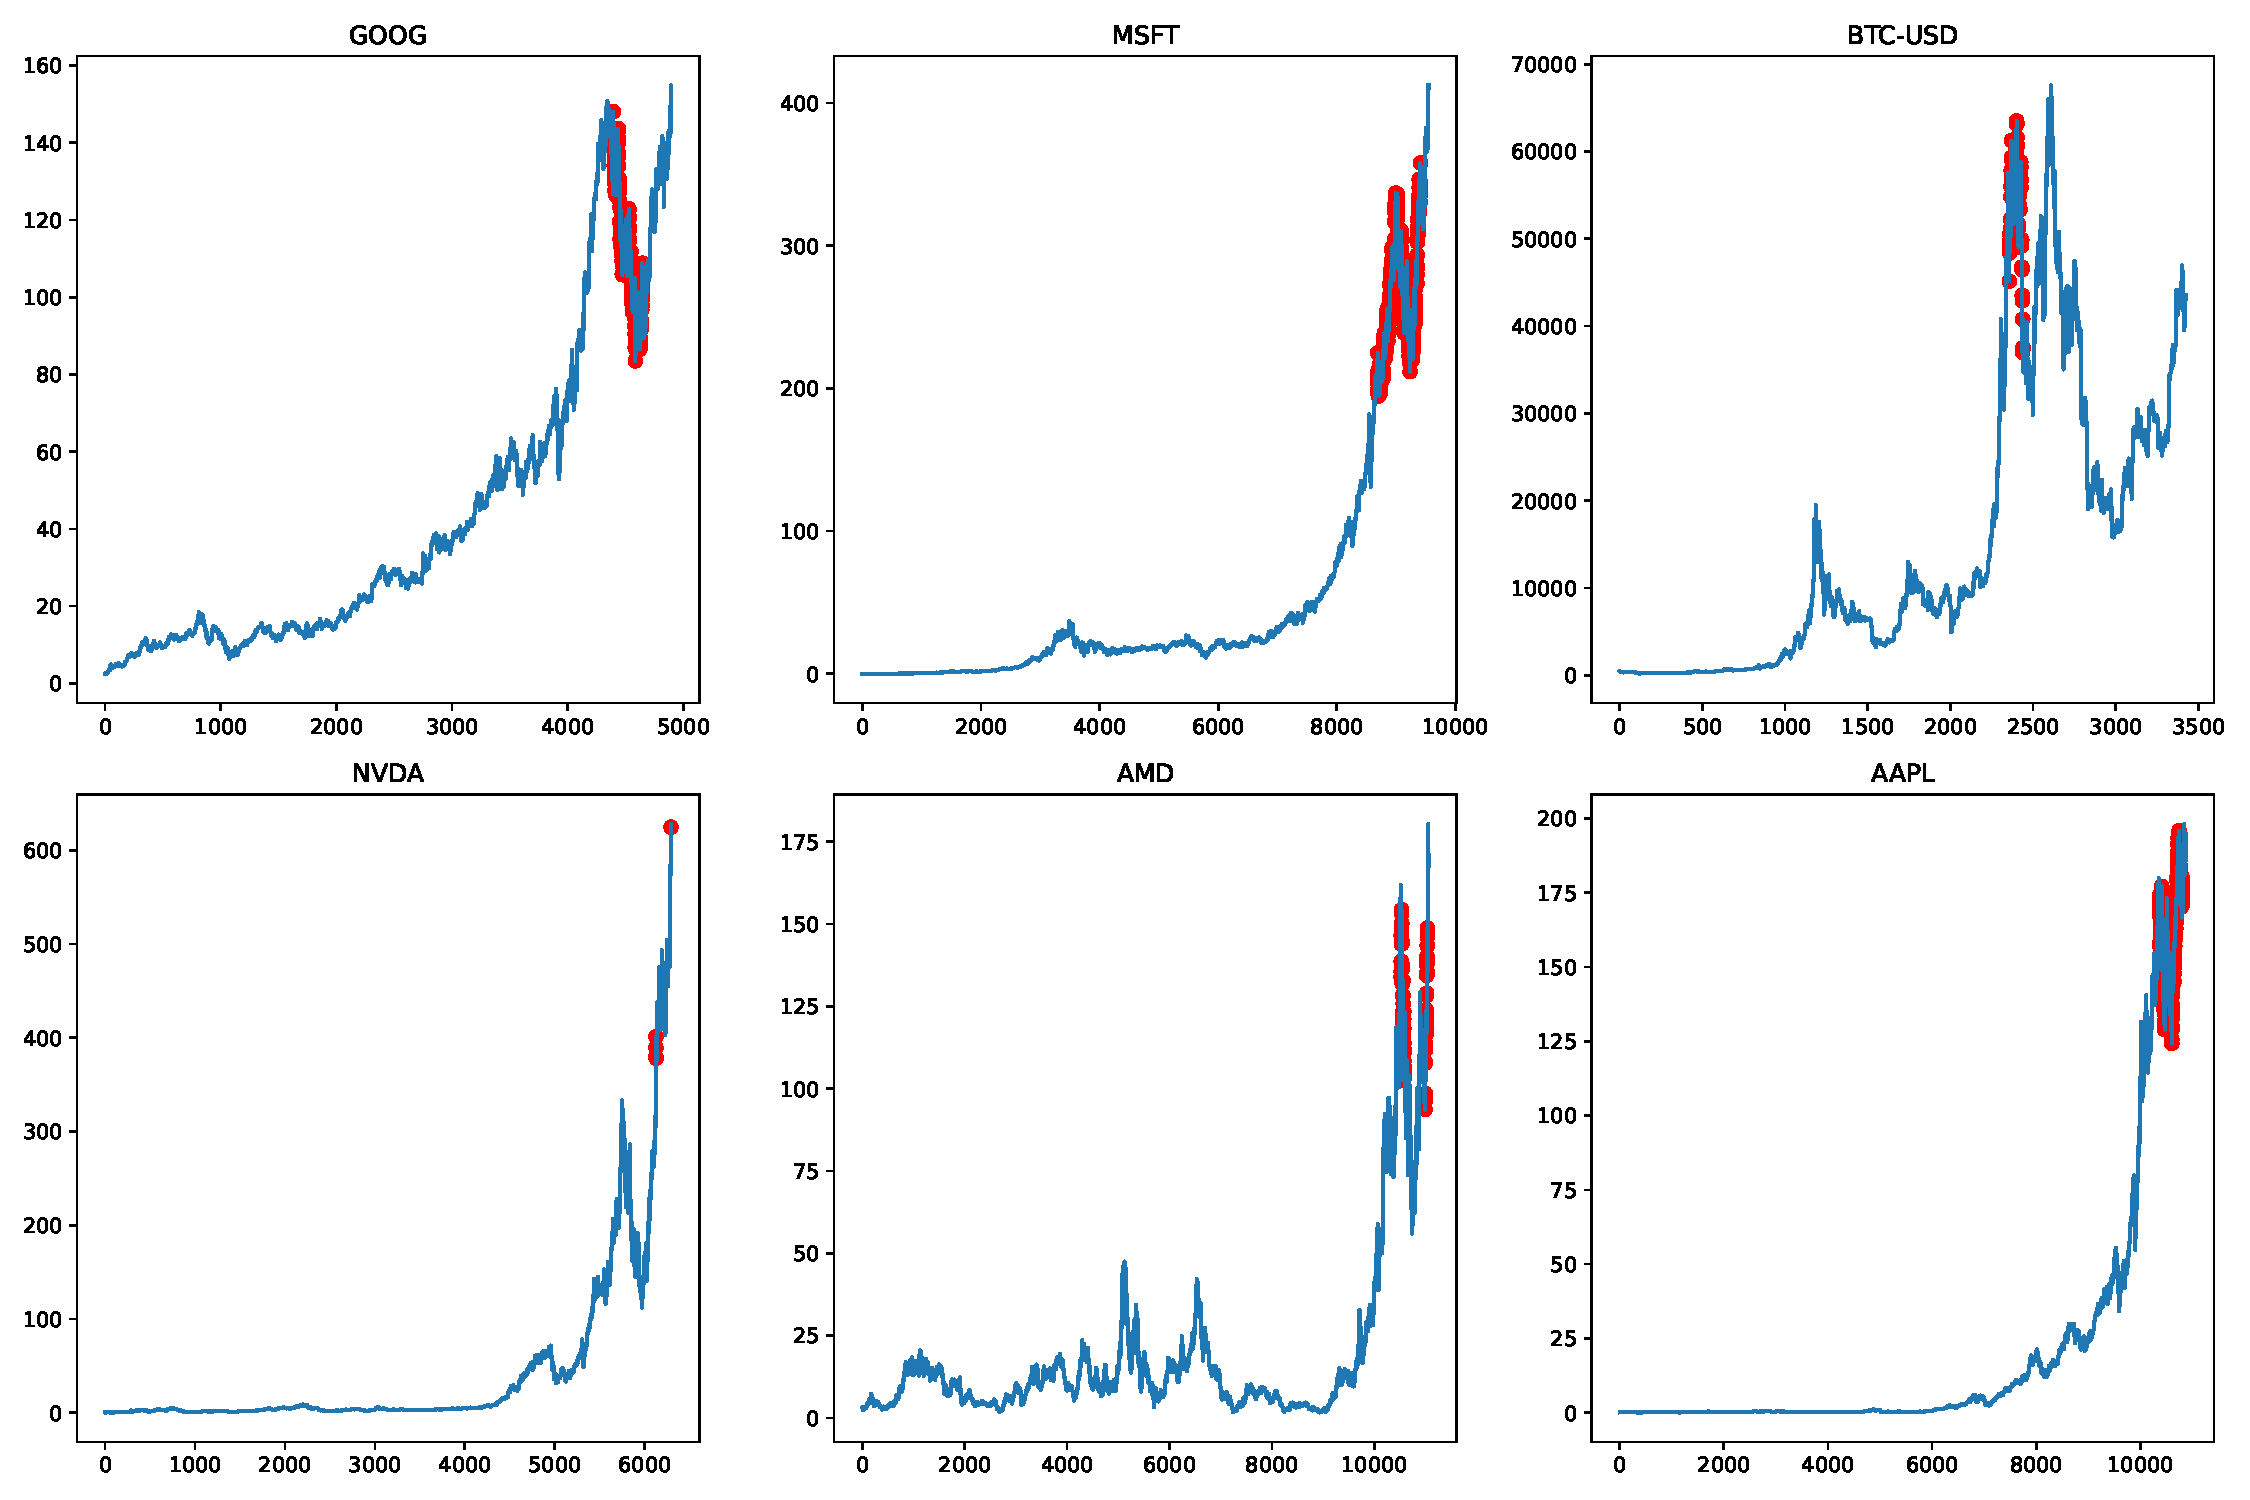
\includegraphics[width=\linewidth]{images/fft_results.pdf}